\documentclass[spanish, fleqn]{article}
\usepackage{babel}
\usepackage[utf8]{inputenc}
\usepackage{amsmath,amsfonts}
\usepackage{enumitem}
\usepackage[colorlinks, urlcolor=blue]{hyperref}
\usepackage{fourier}
\usepackage{tikz}
\usetikzlibrary{shapes.geometric}
\usetikzlibrary{positioning}
\usepackage{verbatim}
\usepackage[top = 2.5cm, bottom = 2cm, left = 2.5cm, right = 2.5cm]{geometry}

\newcommand{\num}{3}

\title{Estructuras Discretas \\
	Tarea \#\num \\
	``TLUITO GAIENL''}
\author{Andrés Navarro\\(201673001-K)}

\begin{document}
	\maketitle
	\thispagestyle{empty}
	
	% Pregunta 1
	\section*{Pregunta 1}
	
	Se tiene un pentágono regular y 3 colores diferentes para colorear su vértices. Calcule el número de maneras de colorear el péntagono, considerando que no es necesario usar todos los colores para cada coloreo y que se consideran equivalentes dos maneras de colorear si resultan iguales al rotar el pentágono.
	
	\begin{center}	
		\begin{minipage}{.22\textwidth}
			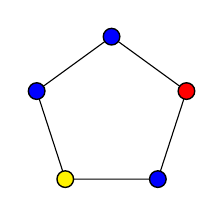
\begin{tikzpicture}
				\draw (90:1cm) -- (18:1cm) -- (306:1cm) -- (234:1cm) -- (162:1cm) -- (90:1cm);
				\draw[line width=.5pt,fill=blue] (90:1cm) circle (3pt);
				\draw[line width=.5pt,fill=red] (18:1cm) circle (3pt);
				\draw[line width=.5pt,fill=blue] (306:1cm) circle (3pt);
				\draw[line width=.5pt,fill=yellow] (234:1cm) circle (3pt);
				\draw[line width=.5pt,fill=blue] (162:1cm) circle (3pt);
			\end{tikzpicture}
		\end{minipage}	
		\begin{minipage}{.14\textwidth}
			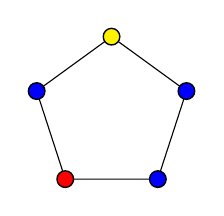
\begin{tikzpicture}
				\draw (90:1cm) -- (18:1cm) -- (306:1cm) -- (234:1cm) -- (162:1cm) -- (90:1cm);
				\draw[line width=.5pt,fill=yellow] (90:1cm) circle (3pt);
				\draw[line width=.5pt,fill=blue] (18:1cm) circle (3pt);
				\draw[line width=.5pt,fill=blue] (306:1cm) circle (3pt);
				\draw[line width=.5pt,fill=red] (234:1cm) circle (3pt);
				\draw[line width=.5pt,fill=blue] (162:1cm) circle (3pt);
			\end{tikzpicture}
		\end{minipage}
	\end{center}
	\begin{center}
		Figura 1: ejemplo de 2 maneras de colorear equivalentes
	\end{center}

	\hfill (30 ptos.)
	
	%% Pregunta 2
	\section*{Pregunta 2}
	Considere la palabra \texttt{EFERVESCENTEMENTE}:
    \begin{enumerate}
    \item ¿De cuántas maneras se pueden ordenar las letras de \texttt{EFERVESCENTE}?
    \item ¿De cuántas maneras se pueden ordenar las letras de \texttt{ME\textsubscript{1}NTE\textsubscript{2}}?
    \item Mapee los ordenamientos de \texttt{ME\textsubscript{1}NTE\textsubscript{2}} a \texttt{MENTE}, ¿qué clase de mapa es este?
    \item ¿Qué clase de mapa es el que lleva de \texttt{E\textsubscript{1}FE\textsubscript{2}RVE\textsubscript{3}SCE\textsubscript{4}NTE\textsubscript{5}ME\textsubscript{6}NTE\textsubscript{7}} a  \texttt{EFERVESCENTEMENTE}?
    \item ¿Cuántos ordenamientos de \texttt{E\textsubscript{1}FE\textsubscript{2}RVE\textsubscript{3}SCE\textsubscript{4}N\textsubscript{1}T\textsubscript{1}E\textsubscript{5}ME\textsubscript{6}N\textsubscript{2}T\textsubscript{2}E\textsubscript{7}} hay?
    \item ¿De cuántas maneras se pueden ordenar sus letras si se quiere que comience o termine con la letra \texttt{T}?
    \end{enumerate}
    
    
	\hfill (40 ptos.)
	
	%% Pregunta 3
	\section*{Pregunta 3}
    Si un tipo de código de barra se compone de 2 letras 
    (del alfabeto inglés de 26 letras), seguido de 3 números 
    y finalmente 2 letras. ¿Cuántos código de barra se pueden
    crear si...
    
    \begin{enumerate}
    	\item Las repeticiones están permitidas.
        \item Las repeticiones no están permitidas.
        \item El código de barras tiene al menos una letra repetida.
    \end{enumerate}
	
	
	\hfill (30 ptos.)\\
	
	
	\vfill\hfill DSW/\LaTeXe
\end{document}
